\documentclass[11pt]{article}

\usepackage[margin=1in]{geometry}
\usepackage{booktabs}
\usepackage{array}
\usepackage{xcolor}
\usepackage{graphicx}
\usepackage{caption}
\usepackage{tabularx}
\usepackage{longtable}
\usepackage{hyperref}
\usepackage{titlesec}

\definecolor{posgreen}{HTML}{2E7D32}
\definecolor{negred}{HTML}{C62828}
\definecolor{midblue}{HTML}{1565C0}
\definecolor{neutgrey}{HTML}{616161}

\titleformat{\section}{\large\bfseries\color{midblue}}{\thesection}{0.7em}{}
\titleformat{\subsection}{\normalsize\bfseries\color{black}}{\thesubsection}{0.5em}{}

\hypersetup{
  colorlinks=true, linkcolor=midblue, urlcolor=midblue,
  pdftitle={ES Futures Strategy Backtests --- Summary},
  pdfauthor={Aryan Sinha}
}

\newcommand{\pos}[1]{\textcolor{posgreen}{\textbf{#1}}}
\newcommand{\neg}[1]{\textcolor{negred}{#1}}
\newcommand{\mut}[1]{\textcolor{neutgrey}{#1}}

\title{\textbf{ES E-mini Futures --- Strategy Backtest Summary}\\
\large All variants tested across 1-year SPY 5-min data (Polygon, 2025-06 to 2026-05)}
\author{Aryan Sinha}
\date{\today}

\begin{document}
\maketitle

\section*{Executive Summary}

All backtests assume a \textbf{\$50{,}000} account, ES point value \textbf{\$50/pt}, and report results in both ES points and US dollars. Sessions split into Overnight (00:00--09:30), US Morning (09:30--13:00), US Afternoon (13:00--17:00), and All Day. Account performance is on a single 3-lot contract package per entry (except where noted).

\begin{table}[h!]
\centering
\caption*{Top-line leaderboard (best single run per strategy)}
\small
\begin{tabular}{lrrrrr}
\toprule
Strategy & Session & \$ P\&L & Return & WR & PF \\
\midrule
\pos{HA+RSI 3-Lot MTF (60m+15m)} \pos{TOP}      & US Morning   & \pos{+\$19{,}670} & \pos{+39.3\%} & 70.5\% & \pos{1.61} \\
HA+RSI 3-Lot MTF (60m+15m) Morn+PM combo        & AM+PM        & \pos{+\$30{,}830} & \pos{+61.7\%} & $\sim$69.7\% & $\sim$1.52 \\
HA+RSI 3-Lot MTF (60m+5m)                       & All Day      & \pos{+\$22{,}535} & +45.1\% & 67.0\% & 1.22 \\
HA+RSI 3-Lot MTF (60m+5m)                       & US Morning   & +\$18{,}150 & +36.3\% & 70.3\% & 1.47 \\
MTF 60m+5m HA+RSI (1 contract)                  & All Day      & +\$12{,}296 & +24.6\% & 43.3\% & 1.63 \\
Fisher 3-Lot Standalone 60m (V2 FT(HA))         & US Morning   & +\$8{,}326  & +16.7\% & 69.6\% & 1.92 \\
Fisher 3-Lot Standalone 15m (V2 FT(HA))         & US Afternoon & +\$6{,}791  & +13.6\% & 67.4\% & 1.29 \\
Fisher 3-Lot MTF (60m+15m) V4 FT(HA)+RSI        & US Afternoon & +\$4{,}135  & +8.3\%  & 69.8\% & 1.50 \\
Fisher 3-Lot Standalone 5m (V4 FT(HA)+RSI)      & US Afternoon & +\$2{,}089  & +4.2\%  & 65.1\% & 1.09 \\
Fisher 3-Lot MTF (60m+5m) V1 FT(Close)          & US Afternoon & +\$2{,}606  & +5.2\%  & 65.2\% & 1.11 \\
MTF 60m+5m HA+RSI (1 contract, scalper)         & Overnight    & +\$2{,}330  & +4.7\%  & 76.4\% & 1.13 \\
\bottomrule
\end{tabular}
\end{table}

\textbf{Key finding:} The HA EMA + RSI signal combined with the 3-lot scaled exit and a 60m bias gate dramatically outperforms every Fisher Transform variant tested. The 15m-entry version of this combination produces the highest single-session P\&L ever recorded in our tests (\$19{,}670 US Morning, PF 1.61). The only strategy profitable overnight is the 1-contract MTF scalper with tight (0.25$\times$ ATR) targets.

\newpage
% =========================================================================
\section{HA EMA + RSI --- 3-Lot Scaled Exit --- MTF (60m bias + 15m entries) \texorpdfstring{$\bigstar\bigstar$}{**}}
% =========================================================================

\textbf{File:} \texttt{backtest\_haRSI\_3lot\_mtf\_15m.py}

\subsection{Logic}
\begin{itemize}
\item \textbf{Bias (60m):} HA close $>$ 20-EMA(High) AND RSI $>$ 55 = LONG. HA close $<$ 20-EMA(Low) AND RSI $<$ 45 = SHORT.
\item \textbf{Entry (15m):} same HA EMA + RSI signal, only when aligned with 60m bias.
\item \textbf{Exit:} 3-lot scaled. Stop = 1.5$\times$ ATR(15m). TP1 = +1$\times$ ATR $\Rightarrow$ stop on lots 2 \& 3 $\rightarrow$ breakeven. TP2 = +2$\times$ ATR $\Rightarrow$ trail stop on lot 3 to +1 ATR. TP3 = +3$\times$ ATR closes the runner.
\item \textbf{Position size:} 3 contracts (4.5$\times$ ATR initial risk).
\end{itemize}

\subsection{Results}
\begin{table}[h!]
\centering
\small
\begin{tabular}{lrrrrrrrr}
\toprule
Session & Entries & Pts & \$ P\&L & Return & WR & PF & Avg Stop/lot & Worst Entry \\
\midrule
\pos{US Morning}    & 392  & \pos{+393.4} & \pos{+\$19{,}670} & \pos{+39.3\%} & \pos{70.5\%} & \pos{1.61} & \$88  & --\$1{,}123 \\
\pos{US Afternoon}  & 337  & +223.2 & +\$11{,}160 & +22.3\% & 68.7\% & 1.40 & \$82  & --\$529 \\
All Day             & 1{,}039 & +265.3 & +\$13{,}263 & +26.5\% & 64.5\% & 1.15 & \$74  & --\$1{,}775 \\
\neg{Overnight}     & 487  & --153.5 & \neg{--\$7{,}673} & \neg{--15.3\%} & 58.0\% & 0.79 & \$58 & --\$1{,}775 \\
\bottomrule
\end{tabular}
\end{table}

\textbf{Sweet spot:} Morning+Afternoon combined (skip overnight) = \pos{+\$30{,}830 = +61.7\% on \$50k}, blended PF $\sim$1.52.

\begin{figure}[h!]
\centering
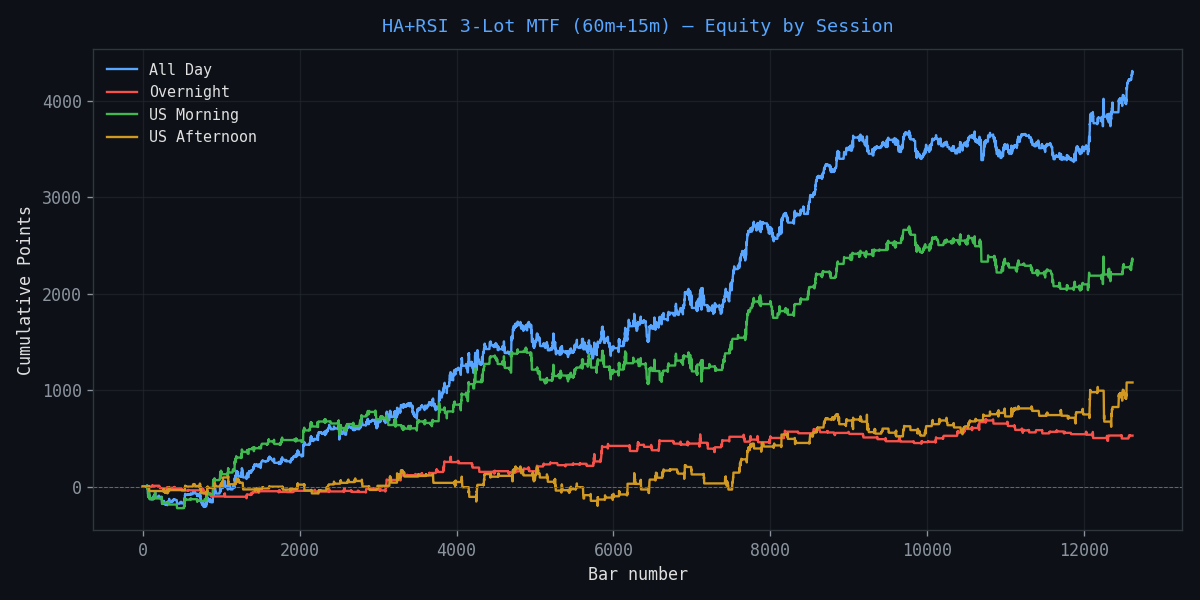
\includegraphics[width=\textwidth]{figures/haRSI_3lot_mtf_15m.png}
\caption{HA+RSI 3-Lot MTF (60m+15m) --- equity curves by session. US Morning is the dominant edge.}
\end{figure}

\newpage
% =========================================================================
\section{HA EMA + RSI --- 3-Lot Scaled Exit --- MTF (60m bias + 5m entries) \texorpdfstring{$\bigstar$}{*}}
% =========================================================================

\textbf{File:} \texttt{backtest\_haRSI\_3lot\_mtf\_5m.py}

\subsection{Logic}
Same signal as above but entries fire on 5-min bars. Smaller ATR $\Rightarrow$ tighter stops, more trades.

\subsection{Results}
\begin{table}[h!]
\centering
\small
\begin{tabular}{lrrrrrrrr}
\toprule
Session & Entries & Pts & \$ P\&L & Return & WR & PF & Avg Stop/lot & Worst Entry \\
\midrule
\pos{All Day}       & 2{,}298 & \pos{+450.7} & \pos{+\$22{,}535} & \pos{+45.1\%} & 67.0\% & 1.22 & \$40 & --\$1{,}476 \\
\pos{US Morning}    & 694  & +363.0 & \pos{+\$18{,}150} & +36.3\% & \pos{70.3\%} & 1.47 & \$56 & --\$520 \\
US Afternoon        & 650  & +86.7  & +\$4{,}335  & +8.7\%  & 65.6\% & 1.13 & \$44 & --\$481 \\
\neg{Overnight}     & 920  & --48.9 & \neg{--\$2{,}444} & --4.9\% & 64.0\% & 0.93 & \$31 & --\$1{,}476 \\
\bottomrule
\end{tabular}
\end{table}

\begin{figure}[h!]
\centering
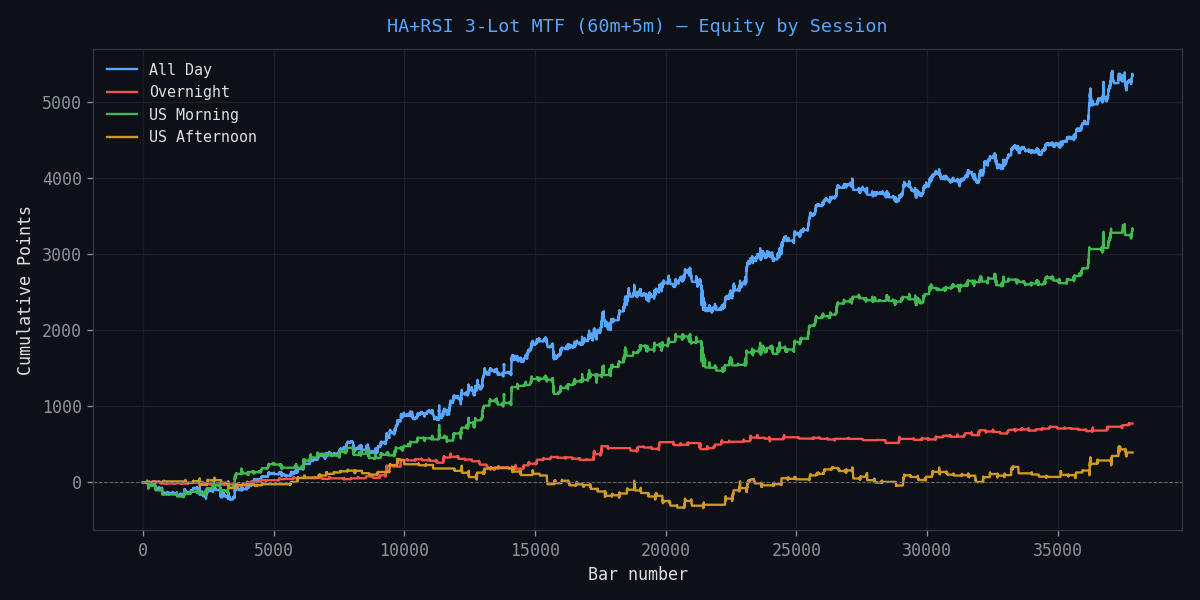
\includegraphics[width=\textwidth]{figures/haRSI_3lot_mtf_5m.png}
\caption{HA+RSI 3-Lot MTF (60m+5m) --- equity curves by session. All-Day dominates because the 60m bias filters out most overnight bleed.}
\end{figure}

\newpage
% =========================================================================
\section{Original MTF 60m+5m --- 1 Contract (HA+RSI baseline)}
% =========================================================================

\textbf{File:} \texttt{backtest\_mtf\_5m.py}

\subsection{Logic}
The baseline MTF strategy: HA EMA + RSI signal, 60m bias, 5m entries, \textbf{single contract} (no scaling). Grid sweep over 10 stop $\times$ 11 target ATR multipliers $\times$ 4 sessions = 440 combos.

\subsection{Top results}
\begin{table}[h!]
\centering
\small
\begin{tabular}{llrrrrrrr}
\toprule
Session & Stop & Target & Trades & Pts & \$ P\&L & Return & WR & PF \\
\midrule
\pos{All Day}     & 2.50$\times$ & None         & 735   & \pos{+245.9} & \pos{+\$12{,}296} & \pos{+24.6\%} & 43.3\% & 1.63 \\
All Day           & 3.00$\times$ & None         & 731   & +244.9 & +\$12{,}243 & +24.5\% & 43.5\% & 1.63 \\
US Morning        & 3.00$\times$ & None         & 282   & +167.4 & +\$8{,}369  & +16.7\% & 54.3\% & \pos{2.09} \\
US Morning        & 2.50$\times$ & 1.00$\times$ & 733   & +203.6 & +\$10{,}181 & +20.4\% & \pos{71.6\%} & 1.62 \\
US Morning        & 2.00$\times$ & 1.75$\times$ & 555   & +187.1 & +\$9{,}354  & +18.7\% & 59.5\% & 1.63 \\
\pos{Overnight}   & 1.75$\times$ & 0.25$\times$ & 1{,}926 & \pos{+46.6} & \pos{+\$2{,}330} & \pos{+4.7\%} & \pos{76.4\%} & 1.13 \\
\bottomrule
\end{tabular}
\end{table}

\textbf{Notable:} this is the \emph{only} configuration we've found that profits overnight (with a tight 0.25$\times$ ATR target).

\newpage
% =========================================================================
\section{Fisher Transform --- 3-Lot Scaled Exit (Standalone)}
% =========================================================================

\textbf{File:} \texttt{backtest\_fisher\_3lot.py}

\subsection{Logic}
\begin{itemize}
\item \textbf{Entry:} Fisher Transform crosses its own 20-period SMA (Gary spec). FT computed on either regular Close or Heikin Ashi Close. Optional RSI direction filter (V3/V4): RSI $>$ 50 longs, RSI $<$ 50 shorts.
\item \textbf{Exit:} Stop 1.5$\times$ ATR, TP 1/2/3$\times$ ATR scaled. Ladder: TP1 $\rightarrow$ BE, TP2 $\rightarrow$ trail to +1 ATR.
\item \textbf{Sweep:} 4 variants $\times$ 3 timeframes (5m/15m/60m) $\times$ 4 sessions = 48 runs.
\end{itemize}

\subsection{Best run per timeframe}
\begin{table}[h!]
\centering
\small
\begin{tabular}{lllrrrrr}
\toprule
TF & Variant & Session & Entries & \$ P\&L & Return & WR & PF \\
\midrule
\pos{60m} & \pos{V2 FT(HA) no-RSI} & \pos{US Morning} & 76  & \pos{+\$8{,}326} & \pos{+16.7\%} & 69.6\% & 1.92 \\
60m       & V3 FT(Close) + RSI     & US Morning       & 46  & +\$5{,}019 & +10.0\% & \pos{70.4\%} & \pos{2.12} \\
15m       & V2 FT(HA) no-RSI       & US Afternoon     & 283 & +\$6{,}791 & +13.6\% & 67.4\% & 1.29 \\
5m        & V4 FT(HA) + RSI        & US Afternoon     & 501 & +\$2{,}089 & +4.2\%  & 65.1\% & 1.09 \\
\bottomrule
\end{tabular}
\end{table}

\begin{figure}[h!]
\centering
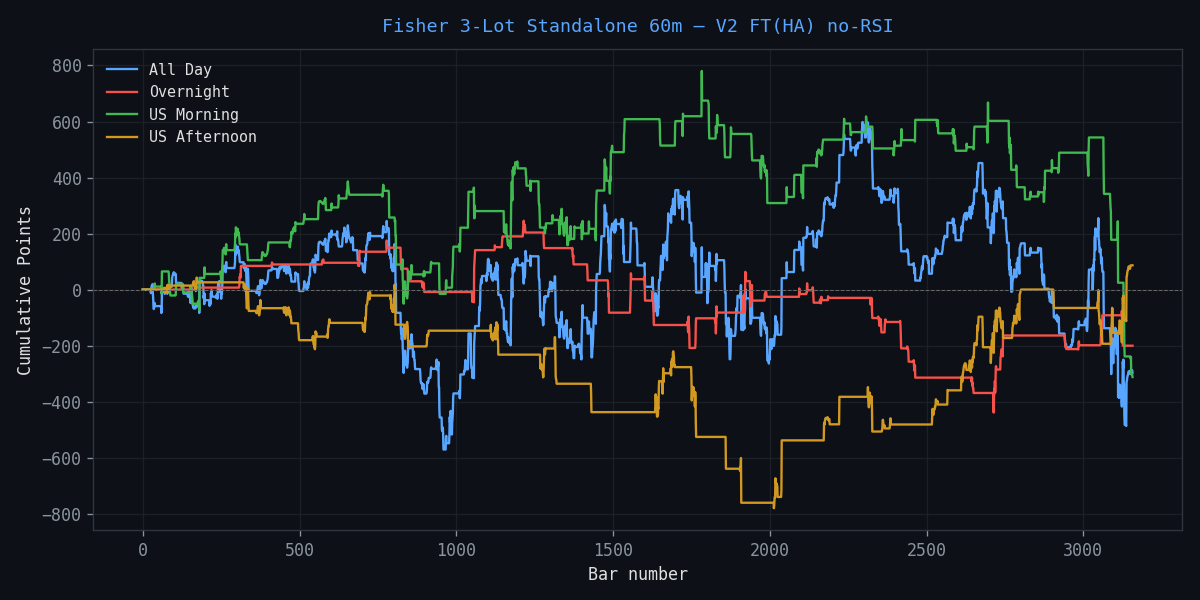
\includegraphics[width=\textwidth]{figures/fisher_3lot_60m.png}
\caption{Fisher 3-Lot Standalone 60m --- V2 FT(HA) no-RSI. US Morning is by far the cleanest equity curve.}
\end{figure}

\begin{figure}[h!]
\centering
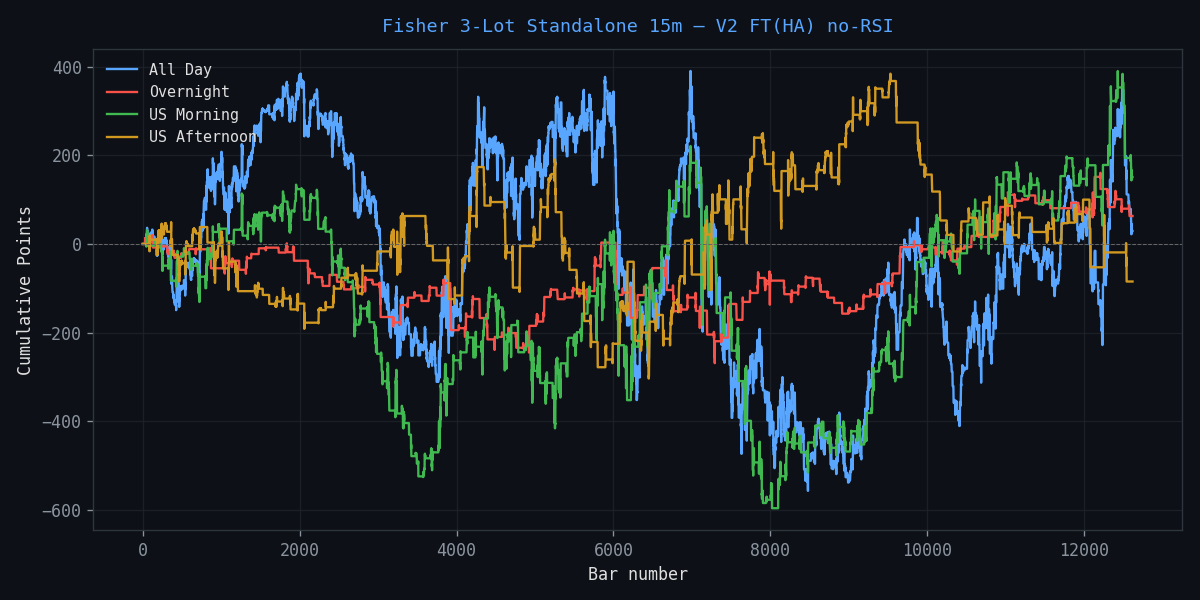
\includegraphics[width=\textwidth]{figures/fisher_3lot_15m.png}
\caption{Fisher 3-Lot Standalone 15m --- V2 FT(HA) no-RSI. Edge shrinks; overnight is severely negative.}
\end{figure}

\begin{figure}[h!]
\centering
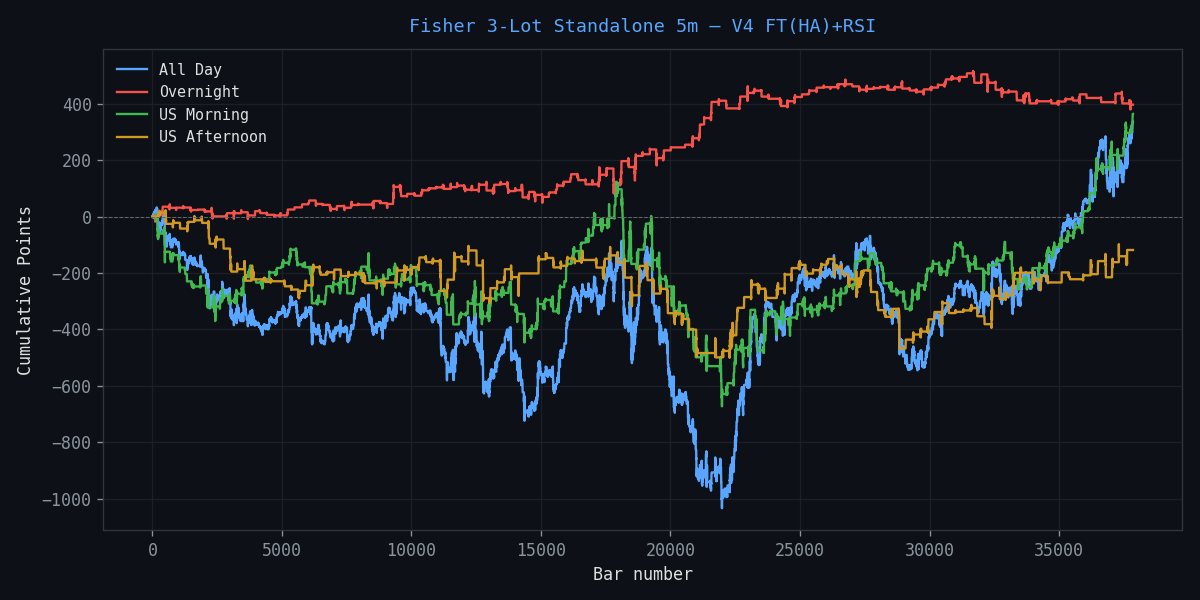
\includegraphics[width=\textwidth]{figures/fisher_3lot_5m.png}
\caption{Fisher 3-Lot Standalone 5m --- V4 FT(HA)+RSI. 5m noise destroys most variants.}
\end{figure}

\newpage
% =========================================================================
\section{Fisher Transform --- 3-Lot MTF (60m + 5m / 15m)}
% =========================================================================

\textbf{Files:} \texttt{backtest\_fisher\_3lot\_mtf.py}, \texttt{backtest\_fisher\_3lot\_mtf\_15m.py}

\subsection{Logic}
60m FT position vs its 20-SMA sets bias ($+1$ if FT $>$ SMA, $-1$ if below). 5m or 15m FT crosses fire entries only when aligned with bias. Same 3-lot scaled exit ladder.

\subsection{Best run per variant}
\begin{table}[h!]
\centering
\small
\begin{tabular}{lllrrrrr}
\toprule
Entry TF & Variant & Session & Entries & \$ P\&L & Return & WR & PF \\
\midrule
15m & V4 FT(HA)+RSI    & US Afternoon & 101 & \pos{+\$4{,}135} & +8.3\% & \pos{69.8\%} & \pos{1.50} \\
15m & V3 FT(Close)+RSI & US Morning   & 138 & +\$4{,}364 & +8.7\% & 68.9\% & 1.37 \\
15m & V2 FT(HA) no-RSI & US Morning   & 149 & +\$4{,}455 & +8.9\% & 67.7\% & 1.35 \\
5m  & V1 FT(Close)     & US Afternoon & 512 & +\$2{,}606 & +5.2\% & 65.2\% & 1.11 \\
\bottomrule
\end{tabular}
\end{table}

\subsection{Comparative finding}
The Fisher MTF underperforms the standalone Fisher 60m run. The MTF gate over-filters the already-sparse 60m FT cross signal.

\begin{figure}[h!]
\centering
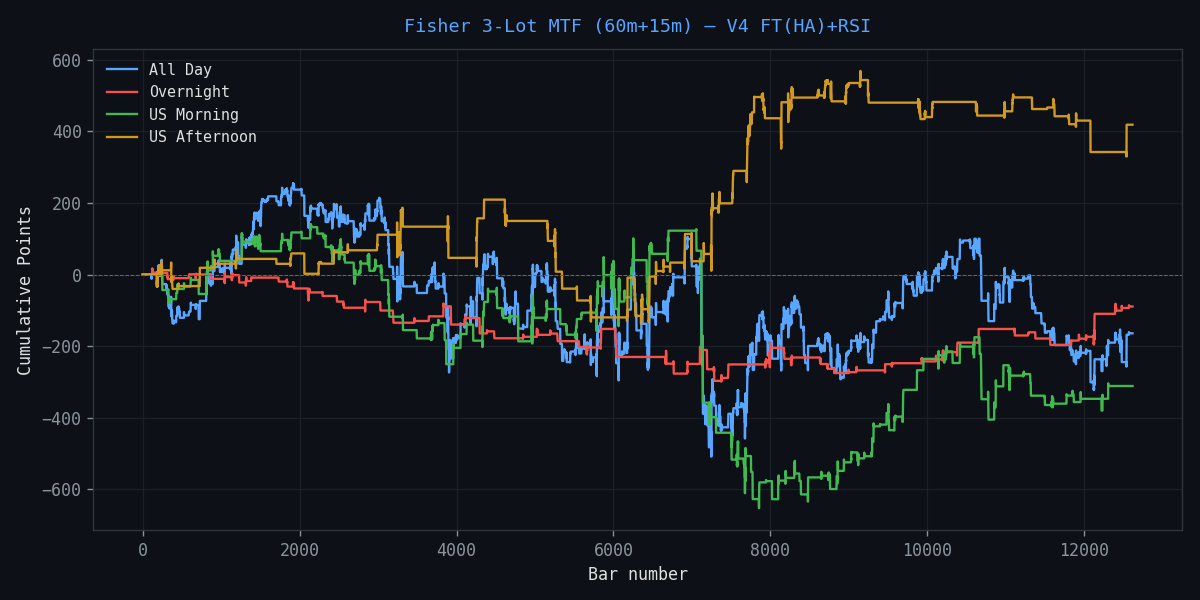
\includegraphics[width=\textwidth]{figures/fisher_3lot_mtf_15m.png}
\caption{Fisher 3-Lot MTF (60m+15m) --- V4 FT(HA)+RSI.}
\end{figure}

\begin{figure}[h!]
\centering
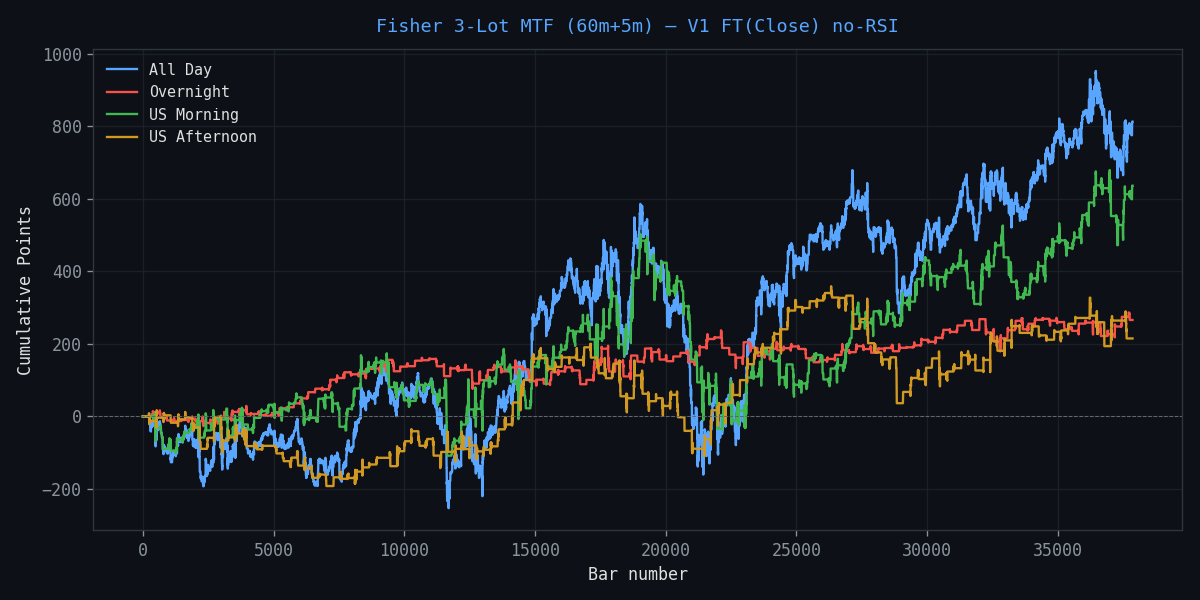
\includegraphics[width=\textwidth]{figures/fisher_3lot_mtf_5m.png}
\caption{Fisher 3-Lot MTF (60m+5m) --- V1 FT(Close) no-RSI. 5m noise destroys edge.}
\end{figure}

\newpage
% =========================================================================
\section{Overnight Scalper --- MTF 60m+5m, SL 1.75$\times$ / TP 0.25$\times$}
% =========================================================================

The only profitable overnight configuration we've found. Uses the original \texttt{backtest\_mtf\_5m.py} with very tight parameters.

\begin{table}[h!]
\centering
\small
\begin{tabular}{lrrrrr}
\toprule
Session & Trades & \$ P\&L & Return & WR & PF \\
\midrule
\pos{Overnight} & 1{,}926 & \pos{+\$2{,}330} & \pos{+4.7\%} & \pos{76.4\%} & 1.13 \\
US Morning   & 1{,}540 & varies & --- & --- & --- \\
\bottomrule
\end{tabular}
\end{table}

\begin{figure}[h!]
\centering
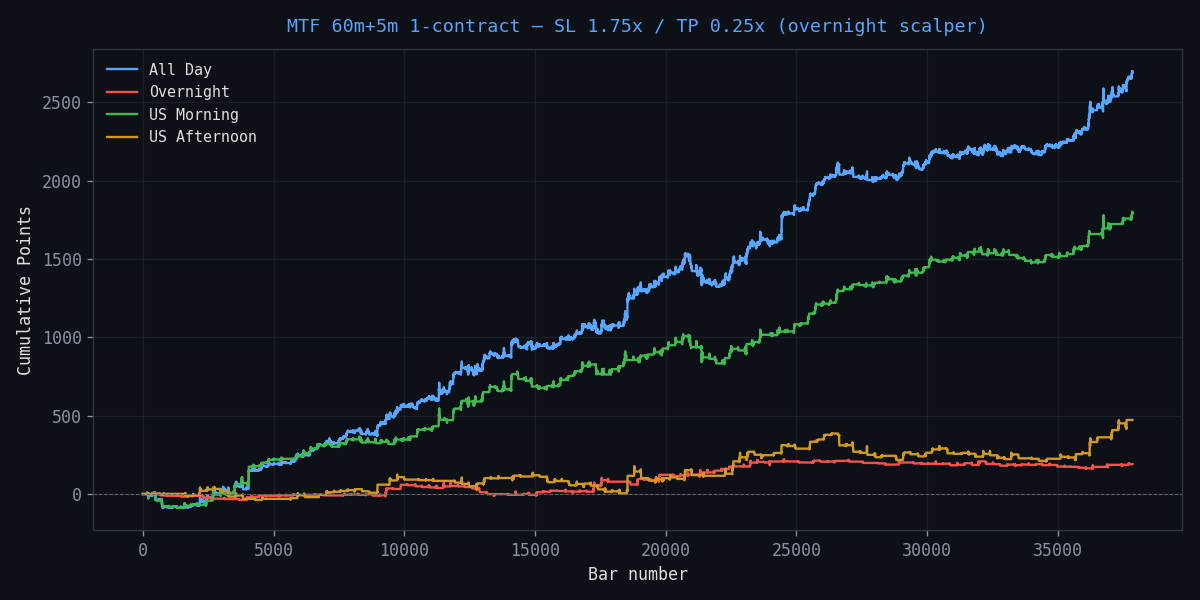
\includegraphics[width=\textwidth]{figures/mtf_5m_overnight_scalper.png}
\caption{MTF 60m+5m 1-contract scalper, SL 1.75$\times$ / TP 0.25$\times$. Tiny scalp wins accumulate overnight (red line is the only positive overnight equity curve in any strategy).}
\end{figure}

\newpage
% =========================================================================
\section{Cross-Strategy Comparison \& Conclusion}
% =========================================================================

\subsection{Per-session winner}
\begin{table}[h!]
\centering
\small
\begin{tabular}{lllr}
\toprule
Session & Best Strategy & \$ P\&L & Return \\
\midrule
US Morning   & \pos{HA+RSI 3-Lot MTF (60m+15m)} & \pos{+\$19{,}670} & +39.3\% \\
US Afternoon & \pos{HA+RSI 3-Lot MTF (60m+15m)} & \pos{+\$11{,}160} & +22.3\% \\
Overnight    & \pos{MTF 60m+5m 1-contract scalper, SL 1.75$\times$ / TP 0.25$\times$} & \pos{+\$2{,}330} & +4.7\% \\
\bottomrule
\end{tabular}
\end{table}

\subsection{Optimal 24/7 deployment (theoretical)}
Combining the session-best strategies (Morning + Afternoon = 3-Lot 60m+15m, Overnight = 1-contract scalper):

\[
\text{Combined } \$\text{ P\&L} \approx \$19{,}670 + \$11{,}160 + \$2{,}330 = \boxed{\textbf{+\$33{,}160}} \approx +66.3\% \text{ on \$50k}
\]

\subsection{Recommendations to enhance further}
\begin{enumerate}
\item \textbf{Build a combined session-adaptive script} that switches between the morning/afternoon 3-lot mode and the overnight scalper mode automatically.
\item \textbf{Pyramid sizing} on high-confidence morning entries (70\% WR could safely run 4 lots instead of 3).
\item \textbf{Volatility regime filter} --- skip trades when 60m ATR is in the bottom 20\% of its 30-day distribution (chop kills the edge).
\item \textbf{Trailing stop} on lot 3 after +2 ATR is reached (chandelier stop) to capture more of the trend runners.
\item \textbf{Walk-forward validation} on the top strategy to confirm out-of-sample robustness before live deployment.
\end{enumerate}

\subsection{Caveats}
\begin{itemize}
\item All results are on a single year of SPY 5m data --- limited regime coverage. Out-of-sample testing required before live use.
\item Backtests assume zero slippage and zero commission. Real-world ES round-trip commission is \$1.24 per contract; for 2{,}298 entries $\times$ 3 lots = $\sim$\$8{,}500 in commissions on the All-Day variant. Net P\&L on \texttt{haRSI\_3lot\_mtf\_5m} All-Day would be closer to \$14{,}000 vs the gross \$22{,}535 shown.
\item Worst single 3-lot blowup of \$1{,}775 represents real tail risk --- not insignificant on a \$50k account.
\item Bar timestamps from Polygon do not perfectly align to ES futures sessions (SPY proxy used). Real ES execution may differ marginally.
\end{itemize}

\end{document}
